\documentclass{standalone}
\usepackage{graphicx}	
\usepackage{amssymb, amsmath}
\usepackage{color}

\usepackage{tikz}
\usetikzlibrary{intersections, backgrounds}

\definecolor{light}{RGB}{220, 188, 188}
\definecolor{mid}{RGB}{185, 124, 124}
\definecolor{dark}{RGB}{143, 39, 39}
\definecolor{highlight}{RGB}{180, 31, 180}
\definecolor{gray10}{gray}{0.1}
\definecolor{gray20}{gray}{0.2}
\definecolor{gray30}{gray}{0.3}
\definecolor{gray40}{gray}{0.4}
\definecolor{gray60}{gray}{0.6}
\definecolor{gray70}{gray}{0.7}
\definecolor{gray80}{gray}{0.8}
\definecolor{gray90}{gray}{0.9}
\definecolor{gray95}{gray}{0.95}

\newcommand*{\offset}{0.025}

\begin{document}

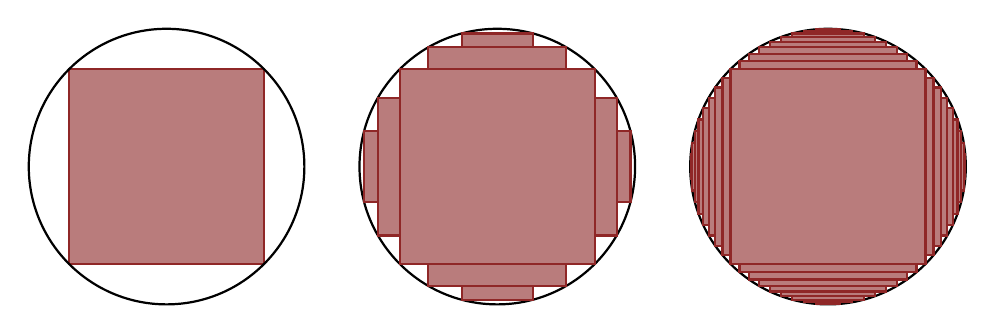
\begin{tikzpicture}[scale=0.35, thick]
  % First Circle
  \draw [color=black] (0, 0) circle (5);

  \filldraw[fill=mid, draw=dark] ({-12 + -5 * cos(45)}, {-5 * cos(45)}) rectangle ({-12 + 5 * cos(45)}, {5 * cos(45)});

  % Second Circle
  \draw [color=black] (-12, 0) circle (5);
  
  \foreach \i in {30, 15} {
    \filldraw[fill=mid, draw=dark] ({-5 * cos(45 + \i)}, 0) rectangle ({5 * cos(45 + \i)}, {5 * sin(45 + \i)});
  } 
  
  \foreach \i in {30, 15} {
    \filldraw[fill=mid, draw=dark] (0, {-5 * cos(45 + \i)}) rectangle ({5 * sin(45 + \i)}, {5 * cos(45 + \i)});
  }   
  
  \foreach \i in {30, 15} {
    \filldraw[fill=mid, draw=dark] ({-5 * cos(45 + \i)}, 0) rectangle ({5 * cos(45 + \i)}, {-5 * sin(45 + \i)});
  }  

  \foreach \i in {30, 15} {
    \filldraw[fill=mid, draw=dark] (0, {-5 * cos(45 + \i)}) rectangle ({-5 * sin(45 + \i)}, {5 * cos(45 + \i)});
  }   

  \filldraw[fill=mid, draw=dark] ({-5 * cos(45)}, {-5 * cos(45)}) rectangle ({5 * cos(45)}, {5 * cos(45)});

  % Third Circle
  \draw [color=black] (12, 0) circle (5);
  
    \foreach \i in {40, 35, ..., 5} {
    \filldraw[fill=mid, draw=dark] ({12 + -5 * cos(45 + \i)}, 0) rectangle ({12 + 5 * cos(45 + \i)}, {5 * sin(45 + \i)});
  } 
  
  \foreach \i in {40, 35, ..., 5} {
    \filldraw[fill=mid, draw=dark] (12, {-5 * cos(45 + \i)}) rectangle ({12 + 5 * sin(45 + \i)}, {5 * cos(45 + \i)});
  }   
  
  \foreach \i in {40, 35, ..., 5} {
    \filldraw[fill=mid, draw=dark] ({12 + -5 * cos(45 + \i)}, 0) rectangle ({12 + 5 * cos(45 + \i)}, {-5 * sin(45 + \i)});
  }  

  \foreach \i in {40, 35, ..., 5} {
    \filldraw[fill=mid, draw=dark] (12, {-5 * cos(45 + \i)}) rectangle ({12 + -5 * sin(45 + \i)}, {5 * cos(45 + \i)});
  }   

  \filldraw[fill=mid, draw=dark] ({12 + -5 * cos(45)}, {-5 * cos(45)}) rectangle ({12 + 5 * cos(45)}, {5 * cos(45)});
  
\end{tikzpicture}

\end{document}  